\section{Example Chapter}

\subsection{Introduction}

This chapter demonstrates the use of images and bibliography in pdfLaTeX documents with best practices.

\subsection{Image References}

Figure~\ref{fig:test_image_pdf} shows a test image. This image is loaded using relative path reference through \texttt{graphicspath} configuration.

\begin{figure}[htbp]
    \centering
    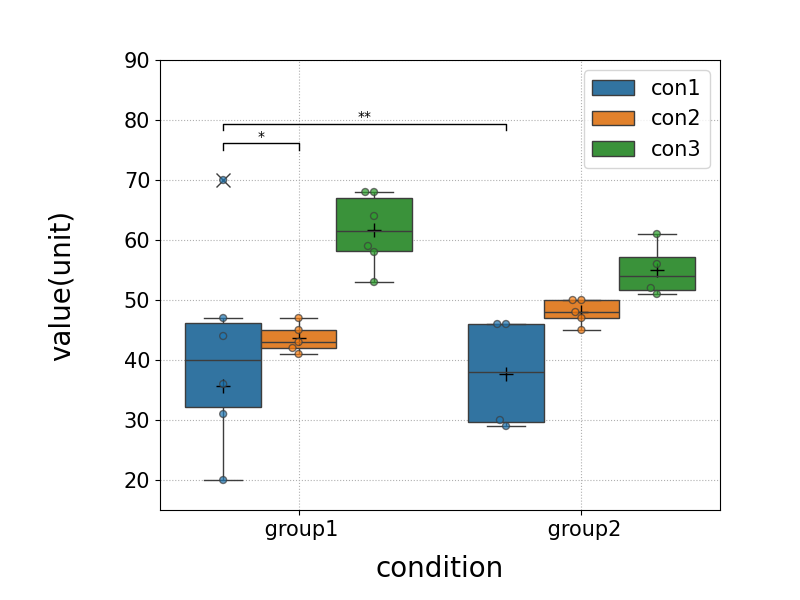
\includegraphics[width=0.6\textwidth]{test/test.png}
    \caption{Example test image}
    \label{fig:test_image_pdf}
\end{figure}

The image path is resolved automatically using the \texttt{\textbackslash graphicspath} setting in the preamble, following best practices.

\subsection{Bibliography Citations}

This section demonstrates bibliography citation examples. For instance, we reference the work by Doe~\cite{example}.

Bibliography management is handled automatically through .latexmkrc configuration.

\subsection{Summary}

This chapter implements LaTeX document creation best practices including:

\begin{itemize}
    \item Image path management with \texttt{graphicspath}
    \item Portability through relative path references
    \item BibTeX bibliography management
\end{itemize}
